% !TeX root = ../main.tex
% !Mode:: "TeX:UTF-8"
\section{第六章 财务分析与融资计划}\label{ux7b2cux516dux7ae0-ux8d22ux52a1ux5206ux6790ux4e0eux878dux8d44ux8ba1ux5212}

PI OS 以企业部署适配、年度产品服务与持续维护为主要商业化方向。财务测算以客户付费和标准化交付为核心，不以科研经费、免费测试规模或行业市场规模直接替代未来经营收入。

现有盖章科研合作协议约定研发经费为 113.3 万元（含税），其中不含税金额 110 万元、税额 3.3 万元。该合同属于华为与天津大学之间的科研合作安排，科研收支与未来创业经营收支分别管理。后续商业化还需结合协议约定完成成果权属、使用范围和必要授权核查。

本章以 2027 年作为商业交付测算起点。2027---2029 年的客户数量、价格、人员配置与融资规模均为基于当前产品规划形成的情景测算，后续将根据实际订单、报价、交付成本和回款情况滚动调整。

\subsection{6.1 基本会计与测算假设}\label{ux57faux672cux4f1aux8ba1ux4e0eux6d4bux7b97ux5047ux8bbe}

未来经营主体拟按照《企业会计准则》建立核算制度，以人民币为记账本位币，按公历年度编制财务信息。为保证经营测算可复核，本章统一采用以下口径：

\begin{quote}
2026 年定位为研发验证和创业筹备期，科研项目收支与未来创业经营收支分开管理，不将已有科研经费转列为公司营业收入。

暂以 2027 年完成必要商用授权并启动商业交付为测算起点；营业收入按不含增值税金额列示，合同金额、会计收入与实际现金回款分别统计。

2027---2029 年年初设备购置预算分别为 10 万元、3 万元和 5 万元，按 5 年直线法、预计净残值为零测算，年度折旧分别为 2.00 万元、2.60 万元和 3.60 万元。

人员预算按 4 人、5 人、6 人的年度平均全职等效规模（FTE）测算，每人每月综合雇佣成本暂按 2 万元计，年度人员预算分别为 96 万元、120 万元和 144 万元。

客户回款按当年收入的 85\% 当年收回、14\% 次年收回、1\% 最终无法收回进行现金需求测算；新增项目优先争取预付款或分阶段付款。
\end{quote}

研发投入主要用于核心功能完善、国产运行环境适配、测试验证、部署工具和维护文档建设。研究阶段支出按当期投入考虑；软件、专利或技术许可只有在经营主体拥有或控制相关权利并满足资产确认条件时，才纳入无形资产核算。设备购置进入现金流测算，设备折旧进入经营测算，避免重复计入。

由于未来经营主体、纳税人类型和交易结构尚未最终确定，本章三年经营表采用税费前口径。正式商业化后，将依据实际合同与主体情况核算企业所得税、增值税及相关附加税费。

\begin{longtable}[]{@{}
  >{\raggedright\arraybackslash}p{(\linewidth - 0\tabcolsep) * \real{1.0000}}@{}}
\toprule\noalign{}
\endhead
\bottomrule\noalign{}
\endlastfoot
\rowcolors{1}{WordTableStripe}{white}
数据与政策依据

• 国家统计局：《2025 年城镇单位就业人员年平均工资情况》（2026 年 5 月 15 日）。

• 《中华人民共和国增值税法》（2026 年 1 月 1 日起施行）及财政部、税务总局相关衔接政策。

• 财政部、税务总局关于小型微利企业所得税优惠的现行政策。

• 科研合作经费、成果权属及披露边界以已盖章合作协议和后续授权文件为准。 \\
\end{longtable}

\subsection{6.2 收入预测}\label{ux6536ux5165ux9884ux6d4b}

PI OS 的收入测算采用``部署适配项目数×平均项目单价＋实际服务期限×年度产品服务单价''的方式。部署适配平均单价暂设为 8 万元/项目，年度产品服务平均单价暂设为 6 万元/客户年。2027---2029 年分别完成 4 个、8 个、12 个部署项目，当年实际服务量分别折合 3 个、10 个、22 个完整客户年。托管资源收费、渠道分成、政府补贴等尚未形成稳定依据的收入暂不纳入测算。

\begin{longtable}[]{@{}
  >{\centering\arraybackslash}p{(\linewidth - 8\tabcolsep) * \real{0.2061}}
  >{\raggedright\arraybackslash}p{(\linewidth - 8\tabcolsep) * \real{0.3588}}
  >{\centering\arraybackslash}p{(\linewidth - 8\tabcolsep) * \real{0.1450}}
  >{\centering\arraybackslash}p{(\linewidth - 8\tabcolsep) * \real{0.1450}}
  >{\centering\arraybackslash}p{(\linewidth - 8\tabcolsep) * \real{0.1450}}@{}}
\caption*{表 6-1 PI OS 收入情景测算（单位：万元）}\tabularnewline
\toprule\noalign{}
\rowcolor{WordTableHeader}
\begin{minipage}[b]{\linewidth}\centering
\TableHeaderText{项目}
\end{minipage} & \begin{minipage}[b]{\linewidth}\centering
\TableHeaderText{计算依据}
\end{minipage} & \begin{minipage}[b]{\linewidth}\centering
\TableHeaderText{2027年}
\end{minipage} & \begin{minipage}[b]{\linewidth}\centering
\TableHeaderText{2028年}
\end{minipage} & \begin{minipage}[b]{\linewidth}\centering
\TableHeaderText{2029年}
\end{minipage} \\
\midrule\noalign{}
\endfirsthead
\toprule\noalign{}
\rowcolor{WordTableHeader}
\begin{minipage}[b]{\linewidth}\centering
\TableHeaderText{项目}
\end{minipage} & \begin{minipage}[b]{\linewidth}\centering
\TableHeaderText{计算依据}
\end{minipage} & \begin{minipage}[b]{\linewidth}\centering
\TableHeaderText{2027年}
\end{minipage} & \begin{minipage}[b]{\linewidth}\centering
\TableHeaderText{2028年}
\end{minipage} & \begin{minipage}[b]{\linewidth}\centering
\TableHeaderText{2029年}
\end{minipage} \\
\midrule\noalign{}
\endhead
\bottomrule\noalign{}
\endlastfoot
\rowcolors{1}{WordTableStripe}{white}
部署适配收入 & 交付项目数×8 万元 & 32.00 & 64.00 & 96.00 \\
年度产品服务收入 & 完整客户年数×6 万元 & 18.00 & 60.00 & 132.00 \\
生态合作等其他收入 & 暂不纳入 & 0.00 & 0.00 & 0.00 \\
\rowcolor{TableTotal}\textbf{收入合计} & \textbf{---} & \textbf{50.00} & \textbf{124.00} & \textbf{228.00} \\
\end{longtable}

\begin{quote}
注：``客户年''反映实际服务期限，例如 2 家客户各接受半年服务，合计为 1 个客户年。
\end{quote}

\begin{center}
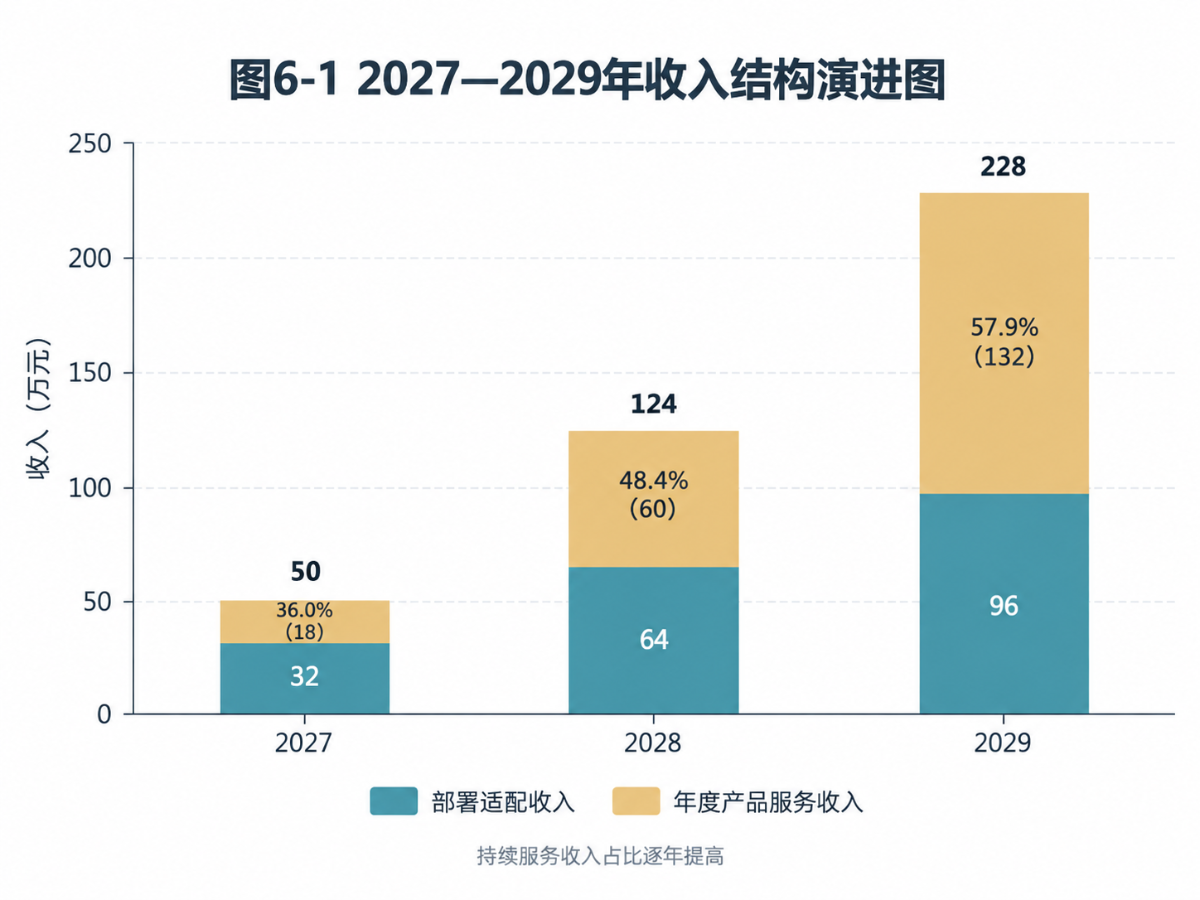
\includegraphics[width=6.15in,height=4.059in]{figures/image21.png}
\end{center}
\WordFigureCaption{图 6-1 2027---2029 年收入结构演进图}

\subsubsection{6.2.1 年度产品服务收入}\label{ux5e74ux5ea6ux4ea7ux54c1ux670dux52a1ux6536ux5165}

年度产品服务拟涵盖经授权的软件使用、版本维护、兼容支持及约定的问题处理。该业务的增长重点不在单次项目数量，而在持续服务能力和客户续费。测算中，年度产品服务收入占比由 2027 年的 36.0\% 提升至 2029 年的 57.9\%，意味着商业模式逐步由一次性部署向持续服务转移。

后续应通过付费试点持续记录价格接受度、支持工时、续费原因和客户流失原因，并据此调整服务边界与年度价格。

\subsubsection{6.2.2 部署适配与生态合作}\label{ux90e8ux7f72ux9002ux914dux4e0eux751fux6001ux5408ux4f5c}

部署适配收入主要来自环境检查、系统接入、安装配置、上线支持和约定培训等工作。测算中的 8 万元为平均项目参数，实际报价应根据客户环境复杂度、改造范围和驻场需求确定，避免以固定低价承接超出标准交付边界的定制需求。

在商用授权和责任边界明确后，PI OS 可进一步探索与软件厂商、云服务商或系统集成商联合交付。现阶段尚未形成稳定分成协议，因此相关收入不进入三年基准测算。

\subsection{6.3 成本分析}\label{ux6210ux672cux5206ux6790}

PI OS 初期以客户自有服务器或云环境部署为主，公司主要承担产品研发、测试验证、交付支持和市场拓展投入，不预设自建大规模公共算力设施。

\begin{longtable}[]{@{}
  >{\centering\arraybackslash}p{(\linewidth - 8\tabcolsep) * \real{0.2217}}
  >{\centering\arraybackslash}p{(\linewidth - 8\tabcolsep) * \real{0.3746}}
  >{\centering\arraybackslash}p{(\linewidth - 8\tabcolsep) * \real{0.1345}}
  >{\centering\arraybackslash}p{(\linewidth - 8\tabcolsep) * \real{0.1345}}
  >{\centering\arraybackslash}p{(\linewidth - 8\tabcolsep) * \real{0.1345}}@{}}
\caption*{表 6-2 PI OS 年度经营投入情景（单位：万元）}\tabularnewline
\toprule\noalign{}
\rowcolor{WordTableHeader}
\begin{minipage}[b]{\linewidth}\centering
\TableHeaderText{成本项目}
\end{minipage} & \begin{minipage}[b]{\linewidth}\centering
\TableHeaderText{预算依据}
\end{minipage} & \begin{minipage}[b]{\linewidth}\centering
\TableHeaderText{2027年}
\end{minipage} & \begin{minipage}[b]{\linewidth}\centering
\TableHeaderText{2028年}
\end{minipage} & \begin{minipage}[b]{\linewidth}\centering
\TableHeaderText{2029年}
\end{minipage} \\
\midrule\noalign{}
\endfirsthead
\toprule\noalign{}
\rowcolor{WordTableHeader}
\begin{minipage}[b]{\linewidth}\centering
\TableHeaderText{成本项目}
\end{minipage} & \begin{minipage}[b]{\linewidth}\centering
\TableHeaderText{预算依据}
\end{minipage} & \begin{minipage}[b]{\linewidth}\centering
\TableHeaderText{2027年}
\end{minipage} & \begin{minipage}[b]{\linewidth}\centering
\TableHeaderText{2028年}
\end{minipage} & \begin{minipage}[b]{\linewidth}\centering
\TableHeaderText{2029年}
\end{minipage} \\
\midrule\noalign{}
\endhead
\bottomrule\noalign{}
\endlastfoot
\rowcolors{1}{WordTableStripe}{white}
人员综合成本 & 4/5/6 名 FTE×24 万元/年 & 96.00 & 120.00 & 144.00 \\
测试、云资源与工具 & 按阶段设置支出上限 & 8.00 & 12.00 & 18.00 \\
市场与客户拓展 & 调研、演示、差旅及渠道活动 & 6.00 & 10.00 & 16.00 \\
办公及专业服务 & 办公、财务、法律等非人工支出 & 8.00 & 10.00 & 14.00 \\
技术许可及第三方支持 & 未取得报价的预留预算 & 8.00 & 12.00 & 16.00 \\
经营性现金支出小计 & 不含设备购置和税费 & 126.00 & 164.00 & 208.00 \\
设备折旧 & 按 6.1 假设计算 & 2.00 & 2.60 & 3.60 \\
信用损失测算 & 当年收入×1\% & 0.50 & 1.24 & 2.28 \\
\rowcolor{TableTotal}\textbf{经营成本合计} & \textbf{用于税费前经营测算} & \textbf{128.50} & \textbf{167.84} & \textbf{213.88} \\
\end{longtable}

\begin{quote}
注：技术许可及第三方支持为预算预留项，后续应根据实际授权方式和报价更新。
\end{quote}

\begin{longtable}[]{@{}
  >{\centering\arraybackslash}p{(\linewidth - 6\tabcolsep) * \real{0.4844}}
  >{\centering\arraybackslash}p{(\linewidth - 6\tabcolsep) * \real{0.1719}}
  >{\centering\arraybackslash}p{(\linewidth - 6\tabcolsep) * \real{0.1719}}
  >{\centering\arraybackslash}p{(\linewidth - 6\tabcolsep) * \real{0.1719}}@{}}
\caption*{表 6-3 收入与经营成本对照（单位：万元）}\tabularnewline
\toprule\noalign{}
\rowcolor{WordTableHeader}
\begin{minipage}[b]{\linewidth}\centering
\TableHeaderText{项目}
\end{minipage} & \begin{minipage}[b]{\linewidth}\centering
\TableHeaderText{2027年}
\end{minipage} & \begin{minipage}[b]{\linewidth}\centering
\TableHeaderText{2028年}
\end{minipage} & \begin{minipage}[b]{\linewidth}\centering
\TableHeaderText{2029年}
\end{minipage} \\
\midrule\noalign{}
\endfirsthead
\toprule\noalign{}
\rowcolor{WordTableHeader}
\begin{minipage}[b]{\linewidth}\centering
\TableHeaderText{项目}
\end{minipage} & \begin{minipage}[b]{\linewidth}\centering
\TableHeaderText{2027年}
\end{minipage} & \begin{minipage}[b]{\linewidth}\centering
\TableHeaderText{2028年}
\end{minipage} & \begin{minipage}[b]{\linewidth}\centering
\TableHeaderText{2029年}
\end{minipage} \\
\midrule\noalign{}
\endhead
\bottomrule\noalign{}
\endlastfoot
\rowcolors{1}{WordTableStripe}{white}
收入 & 50.00 & 124.00 & 228.00 \\
\rowcolor{TableTotal}\textbf{经营成本合计} & \textbf{128.50} & \textbf{167.84} & \textbf{213.88} \\
\rowcolor{TableTotal}\textbf{税费前经营测算结余} & \textbf{-78.50} & \textbf{-43.84} & \textbf{14.12} \\
\end{longtable}

基准情景下，2029 年税费前经营测算结余转正，但前两年的累计投入尚未收回。敏感性测试显示，经营结果对收入兑现和人员成本较为敏感：若 2029 年收入较基准情景下降 20\%，税费前结余约为 -31.02 万元；若 2029 年人员综合成本增加 20\%，结余约为 -14.68 万元。

因此，经营重点应放在提高交付复用率、提升持续服务收入占比，并验证客户是否愿意按能够覆盖完整交付成本的价格采购。

\begin{center}
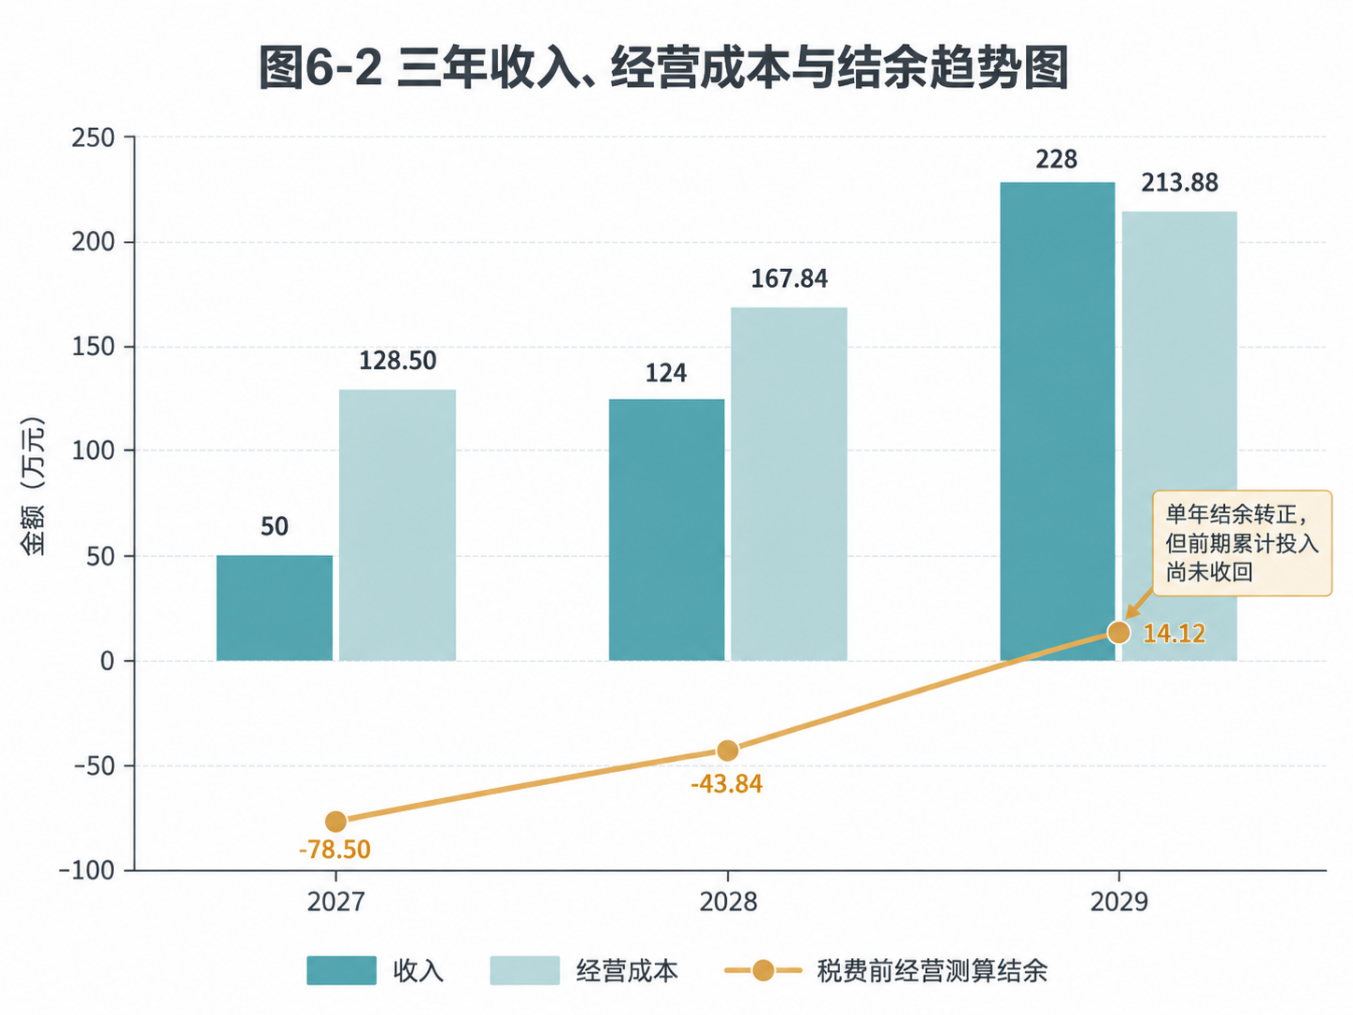
\includegraphics[width=6.15in,height=4.059in]{figures/image22.png}
\end{center}
\WordFigureCaption{图 6-2 三年收入、经营成本与结余趋势图}

\subsection{6.4 融资计划}\label{ux878dux8d44ux8ba1ux5212}

融资需求依据经营性现金缺口推算。按照回款假设，当年客户现金回款=当年收入×85\%＋上年收入×14\%。

\begin{longtable}[]{@{}
  >{\centering\arraybackslash}p{(\linewidth - 6\tabcolsep) * \real{0.4844}}
  >{\centering\arraybackslash}p{(\linewidth - 6\tabcolsep) * \real{0.1719}}
  >{\centering\arraybackslash}p{(\linewidth - 6\tabcolsep) * \real{0.1719}}
  >{\centering\arraybackslash}p{(\linewidth - 6\tabcolsep) * \real{0.1719}}@{}}
\caption*{表 6-4 PI OS 基础现金需求测算（单位：万元）}\tabularnewline
\toprule\noalign{}
\rowcolor{WordTableHeader}
\begin{minipage}[b]{\linewidth}\centering
\TableHeaderText{项目}
\end{minipage} & \begin{minipage}[b]{\linewidth}\centering
\TableHeaderText{2027年}
\end{minipage} & \begin{minipage}[b]{\linewidth}\centering
\TableHeaderText{2028年}
\end{minipage} & \begin{minipage}[b]{\linewidth}\centering
\TableHeaderText{2029年}
\end{minipage} \\
\midrule\noalign{}
\endfirsthead
\toprule\noalign{}
\rowcolor{WordTableHeader}
\begin{minipage}[b]{\linewidth}\centering
\TableHeaderText{项目}
\end{minipage} & \begin{minipage}[b]{\linewidth}\centering
\TableHeaderText{2027年}
\end{minipage} & \begin{minipage}[b]{\linewidth}\centering
\TableHeaderText{2028年}
\end{minipage} & \begin{minipage}[b]{\linewidth}\centering
\TableHeaderText{2029年}
\end{minipage} \\
\midrule\noalign{}
\endhead
\bottomrule\noalign{}
\endlastfoot
\rowcolors{1}{WordTableStripe}{white}
客户现金回款 & 42.50 & 112.40 & 211.16 \\
经营性现金支出 & 126.00 & 164.00 & 208.00 \\
设备购置支出 & 10.00 & 3.00 & 5.00 \\
\rowcolor{TableTotal}\textbf{融资前现金净额} & \textbf{-93.50} & \textbf{-54.60} & \textbf{-1.84} \\
\end{longtable}

\begin{quote}
注：折旧和信用损失准备不重复作为现金支出扣除；表内尚未全面计入税费、押金、保证金及月内收支时差。
\end{quote}

虽然 2029 年税费前经营测算结余转正，融资前现金净额仍为 -1.84 万元，说明项目除关注盈利能力外，还需要管理客户验收和回款节奏。

\subsubsection{6.4.1 首轮资金需求}\label{ux9996ux8f6eux8d44ux91d1ux9700ux6c42}

按照基准情景，2027---2028 年累计基础现金缺口为 148.10 万元。考虑客户回款延迟、授权费用变化、采购时点和交付返工等不确定因素，以基础现金缺口的 20\% 设置安全缓冲，约为 29.62 万元，对应测算资金需求约 177.72 万元。因此，首轮融资目标取整为 180 万元。

\begin{longtable}[]{@{}
  >{\centering\arraybackslash}p{(\linewidth - 2\tabcolsep) * \real{0.7460}}
  >{\centering\arraybackslash}p{(\linewidth - 2\tabcolsep) * \real{0.2540}}@{}}
\caption*{表 6-5 首轮资金需求构成（单位：万元）}\tabularnewline
\toprule\noalign{}
\rowcolor{WordTableHeader}
\begin{minipage}[b]{\linewidth}\centering
\TableHeaderText{项目}
\end{minipage} & \begin{minipage}[b]{\linewidth}\centering
\TableHeaderText{金额}
\end{minipage} \\
\midrule\noalign{}
\endfirsthead
\toprule\noalign{}
\rowcolor{WordTableHeader}
\begin{minipage}[b]{\linewidth}\centering
\TableHeaderText{项目}
\end{minipage} & \begin{minipage}[b]{\linewidth}\centering
\TableHeaderText{金额}
\end{minipage} \\
\midrule\noalign{}
\endhead
\bottomrule\noalign{}
\endlastfoot
\rowcolors{1}{WordTableStripe}{white}
首两年经营性现金支出 & 290.00 \\
首两年设备购置支出 & 13.00 \\
减：预计客户现金回款 & 154.90 \\
基础资金缺口 & 148.10 \\
安全缓冲（基础缺口×20\%） & 29.62 \\
\rowcolor{TableTotal}\textbf{测算资金需求} & \textbf{177.72} \\
首轮融资目标（取整） & 180.00 \\
\end{longtable}

\begin{center}
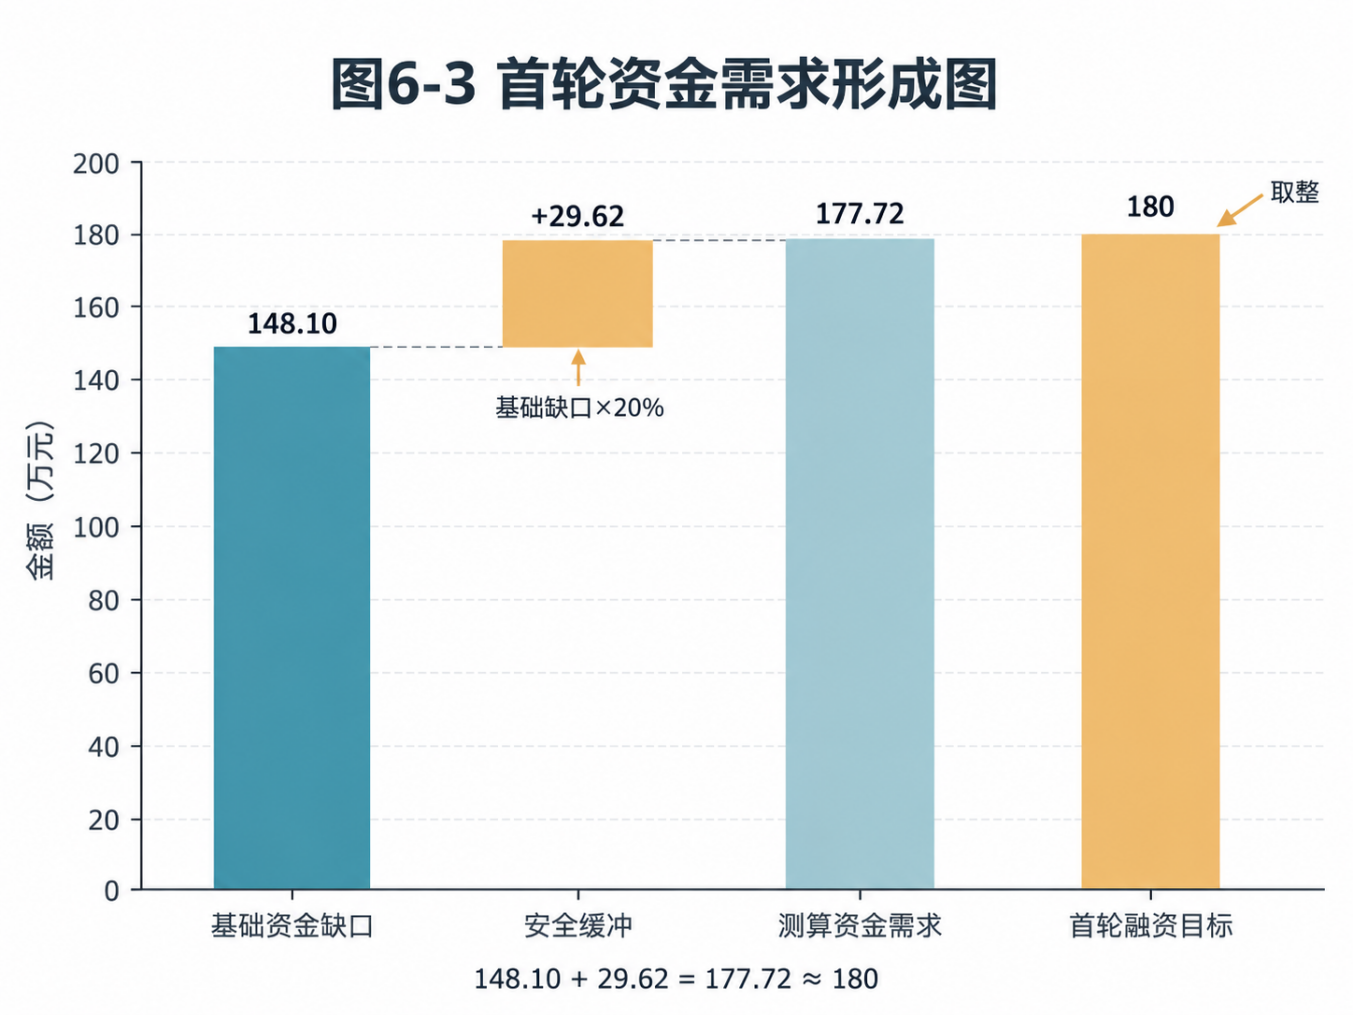
\includegraphics[width=6.15in,height=4.059in]{figures/image23.png}
\end{center}
\WordFigureCaption{图 6-3 首轮资金需求形成图}

\subsubsection{6.4.2 资金使用与分阶段控制}\label{ux8d44ux91d1ux4f7fux7528ux4e0eux5206ux9636ux6bb5ux63a7ux5236}

资金优先用于产品化研发、命题指定环境适配、测试验证、首批客户交付和必要经营保障。正式融资前重点完成以下准备：

\begin{quote}
明确经营主体、成果商用权限以及合作协议中的使用与披露限制。

形成可验收的产品版本、标准交付边界和复现材料。

通过客户访谈、付费试点或订单验证价格、业务量和续费判断。

补齐逐月现金预算、主要采购报价和人员投入计划。
\end{quote}

项目采用分阶段投入方式：产品验收前控制非必要营销投入和人员扩张，形成付费交付后再根据销售与支持瓶颈增加人员。若前两年客户回款较基准情景减少 20\%，将额外占用约 30.98 万元资金，已接近当前安全缓冲上限，因此招聘、设备采购和重大定制项目需要结合现金余额滚动决策。后续融资以可复制交付、续费和回款质量为主要依据；资本退出以战略并购或后续融资中的股权转让为主要可选路径，待业务规模和治理基础成熟后再评估资本市场路径。

